\begin{figure}[htbp]
\centering
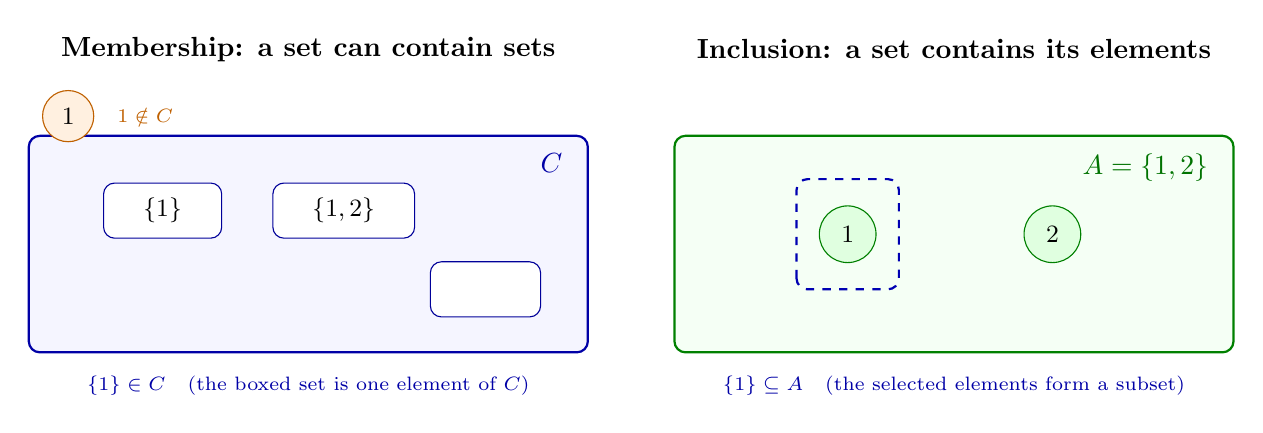
\begin{tikzpicture}[font=\small]
    \node[font=\bfseries] at (3.55,3.85) {Membership: a set can contain sets};
    \draw[rounded corners,thick,draw=blue!65!black,fill=blue!4] (0,0) rectangle (7.1,2.75);
    \node[anchor=north east,font=\bfseries,text=blue!65!black] at (6.9,2.65) {$C$};
    \node[draw=blue!60!black,fill=white,rounded corners,minimum width=1.5cm,minimum height=0.7cm] at (1.7,1.8) {$\{1\}$};
    \node[draw=blue!60!black,fill=white,rounded corners,minimum width=1.8cm,minimum height=0.7cm] at (4.0,1.8) {$\{1,2\}$};
    \node[draw=blue!60!black,fill=white,rounded corners,minimum width=1.4cm,minimum height=0.7cm] at (5.8,0.8) {$\varnothing$};
    \node[draw=orange!75!black,fill=orange!12,circle,minimum size=0.65cm] at (0.5,3.0) {$1$};
    \node[anchor=west,font=\scriptsize,text=orange!75!black] at (1.0,3.0) {$1\notin C$};
    \node[font=\scriptsize,text=blue!65!black] at (3.55,-0.42) {$\{1\}\in C$\quad(the boxed set is one element of $C$)};

    \begin{scope}[xshift=8.2cm]
        \node[font=\bfseries] at (3.55,3.85) {Inclusion: a set contains its elements};
        \draw[rounded corners,thick,draw=green!50!black,fill=green!4] (0,0) rectangle (7.1,2.75);
        \node[anchor=north east,font=\bfseries,text=green!45!black] at (6.9,2.65) {$A=\{1,2\}$};
        \node[draw=green!50!black,fill=green!12,circle,minimum size=0.72cm] (one) at (2.2,1.5) {$1$};
        \node[draw=green!50!black,fill=green!12,circle,minimum size=0.72cm] at (4.8,1.5) {$2$};
        \draw[blue!70!black,dashed,thick,rounded corners] (1.55,0.8) rectangle (2.85,2.2);
        \node[font=\scriptsize,text=blue!65!black] at (3.55,-0.42) {$\{1\}\subseteq A$\quad(the selected elements form a subset)};
    \end{scope}
\end{tikzpicture}
\caption{In $C=\{\{1\},\{1,2\},\varnothing\}$, the set $\{1\}$ is an element but the number $1$ is not. In contrast, $1$ is an element of $A=\{1,2\}$, and the singleton $\{1\}$ is a subset of $A$.}
\label{fig:membership-versus-inclusion}
\end{figure}